\documentclass[11pt,letterpaper]{article}

\usepackage[utf8]{inputenc}
\usepackage{fullpage} % Package to use full page
\usepackage[utf8]{inputenc}
\usepackage{fullpage} % Package to use full page
\usepackage{parskip} % Package to tweak paragraph skipping
\usepackage{tikz} % Package for drawing
\usepackage{amsmath}
\usepackage{amsfonts}
\usepackage{amssymb}
\usepackage{hyperref}
\usepackage{float}
\usepackage[]{algorithm2e}
\usepackage{listings}
\usepackage{tabularx}
\usepackage[spanish,es-nodecimaldot]{babel}


\title {Facultad de Ciencias, UNAM\\
		Proyeto Final\\  
		Modelando un juego de matanza.\\  
		}
\author{Marisol Amézcua Lopez }  

\date{\today}  

\begin{document}

\maketitle

\section{Introducción}

Para el proyecto se tomó como base la historia principal de un juego llamado Danganronpa, en donde parten de tomar a cierto número de personas, encerrarlas y obligarlas a participar en un juego en el que tienen que matarse entre ellos para 
poder salir del recinto, con esta finalidad cada cierto tiempo se les da lo que se llama un incentivo, esto para motivar 
las muertes; sin embargo los participantes pueden optar también por cooperar entre todos. 
Cuando ocurra una muerte los demás participantes tienen que encontrar al culpable, en caso de hallarlo el culpable es ejecutado, de otra manera, todos los demás participantes mueren.

Usando esta premisa se pretende modelar el comportamiento de los agentes y del 
entorno, ver como evolucionan las interacciones y analizar la cadena de sucesos
ocurridos.

\section{Planteamiento}
%Con que se piensa resolver, herramientas, tecnologías, etc
Dado el proble a modelar, es necesario contar con las animaciones para poder observar las interacciones entre los agentes esto con el objetivo de saber qué es lo que 
ocurre con el sistema dadas las reglas del modelo.
Por ello para la implementación del proyecto se piensa usar el software \emph{Processing 3.3.0} y usar el lenguaje Python dentro de este, lo anterior con la finalidad de utilizar sus bibliotecas de animaciones.

\section{Desarrollo}
%Diseños lógicos, algoritmos, diagramas de flujo, especificaciones de la implementación.
Para la estructura se diseñaron dos clases, la clase \textbf{jugador} y la clase
\textbf{tablero}.
En la clase jugador se tienen los siguientes atributos:

\begin{itemize}
	\item Id: El id del jugador.
	\item Posicion: Posición del jugador en el tablero.
	\item Valores máximos en x y y, esto para controlar que no se salga el agente
	de la retícula.
	\item Estado: Vivo o muerto, esto para controlar las muertes en el sistema.
	\item Vecinos: Es una lista de longitud N, donde N es la cantidad de jugadores
	y en cada posición i guarda la afinidad que el agente tiene con el jugador i. Nótese que la afinidad del jugador i con el agente en cuestión puede no ser la
	misma. En la posición que corresponde al id del jugador guardamos un -1, esto 
	también se da si el i-ésimo jugador esta muerto, en otras palabras, hay un -1 en la lista si la posicion i corresponde al id del jugador o bien el i-ésimo jugador está muerto. Estos valores son enteros del 0 al 100 y comienzan con valores aleatorios entre el 40 y 60.
	\item Desesperacion: Corresponde al valor de desesperación del agente, el 
	dominio de este valor va de 0 a 20, al llegar al nivel mas alto el jugador 
	es capaz de asesinar.
	\item Sospechoso: En la fase del juicio el id del posible asesino se guarda en
	esta variable, así podemos saber la cantidad de jugadores que saben quien es el asesino.
\end{itemize}

Por otro lado, en la clase Tablero tenemos lo siguiente:

\begin{itemize}
	\item Tamaño: Tamaños máximos y mínimos de la retícula
	\item Retícula: Malla donde interactúan los agentes, esta malla tiene en 
	la posición i,j el numero k si el agente k se encuentra en la posición i,j.
	Esto para aumentar la eficiencia a la hora de obtener las vecindades y también
	a la hora de animar.
	\item Jugadores: Es una lista que contiene cada objeto jugador que esta participando.
	\item Fase: Fase en la que se encuentra el sistema, estas se explicarán más adelante.
	\item Asesino: Id del asesino en turno.
	\item Asesinado: Id de la víctima.
	\item Posición de la víctima: Posición donde falleció la víctima.
	\item Tiempo restante del juicio: Se trata de un entero que cuenta cuánto queda
	para que termine la fase del juicio.
\end{itemize}

Con lo anterior se arrancó el sistema, el cual se dividió en 3 fases importantes.

\begin{itemize}
	\item {\large \textbf{Fase 0}}:
	
	La fase 0 consiste en la interacción entre los agentes y es la primera fase en 
	la que se encuentra el sistema a la hora de iniciar. Los agentes se mueven de
	forma aleatoria una casilla contigua a ellos utilizando vecindades de Moore.
	En cada iteración se verifica a los jugadores cercanos y se interacciona con 
	ellos, para esto se utilizó la siguiente tabla la cual parte del Dilema del Prisionero\cite{WDil}:
	
	Sea J1, J2 dos jugadores distintos
	
	\begin{tabular}{|c|c|c|}
		\hline 
		& J1: Afinidad Positiva & J1:Afinidad Negativa \\ 
		\hline 
		J2:Afinidad Positiva & J1: +3, J2: +3 & J1: +5, J2: -5 \\ 
		\hline 
		J2:Afinidad Negativa & J1: -5, J2: +5 & J1: -1, J2: -1 \\ 
		\hline 
	\end{tabular} 

	Si la afinidad del jugador 1 con el jugador 2 es mayor o igual a 50 entonces
	la afinidad se considera positiva, en otro caso negativa.
	
	Durante la misma fase se dan los incentivos, los cuales aumentan la desesperación
	de cada jugador, para esto cada 30 iteraciones a la desesperación de todos
	los jugadores se le suma una cantidad aleatoria entre 1 y 3. En la misma fase,
	para cada iteración, ocurre que si el promedio de las afinidades del jugador i es mayor a 50 (el jugador i tiene en promedio una afinidad positiva), entonces la
	desesperación decrementa una cantidad aleatoria entre 0 y 2 puntos. Esto se hizo con la finalidad de modelar que, si uno tiene una interacción positiva 
	con los demás agentes entonces es capaz de sentirse menos corrompido por el entorno. 
	
	
	\item {\large \textbf{Fase 1}}: 
	
	Para pasar a la fase 1 tiene que ocurrir que haya un asesino, en otras palabras, en cuanto un jugador alcance el valor 20 de desesperación.
	Es importante aclarar que solo un asesino a la vez mata, por lo que si hay mas de un jugador con el valor máximo de desesperación entonces tomamos uno de forma aleatoria.
	
	Durante esta fase el asesino en turno busca una víctima, para que un jugador 
	pueda ser víctima tiene que cumplir con estar dentro de la vecindad de Moore del
	asesino.
	
	En cuanto ocurre el asesinato se registra el asesino y la víctima así como la
	posición de la víctima, también se le agrega desesperación a todos los jugadores
	esta adición es un número aleatorio entre 1 y 3.
	
	Una vez con esto se calcula el jugador más cercano a los hechos y ese jugador
	es el que tendrá conocimiento de quién es el culpable.
	
	\item {\large \textbf{Fase 2}}:
	
	Esta fase comprende lo que es el juicio, durante esta fase lo agentes van a propagar quién es el culpable. Para esto los agentes se mueven sobre la retícula
	y cuando entren en contacto con otro agente haran lo siguiente:
	
	Sean J1 y J2 dos jugadores distintos
	\begin{itemize}
		\item Si J1 no tiene sospechoso y J2 sí lo tiene, entonces si la afinidad 
		de J1 con J2 es mayor o igual a 40 J1 le cree a J2 y se propaga el sospechoso.
		\item Si J2 no tiene sospechoso y J1 sí, se aplica la regla anterior.
		\item Si ninguno de los dos tiene sospechoso, no se propaga nada.
	\end{itemize}

	El nivel de afinidad necesario para considerarse positiva en este caso desciende
	dado que los rumores negativos o bien importantes se propagan con más facilidad.
	
	Para propagar el rumor los jugadores tienen un tiempo límite, el cual es el 
	tiempo restante del juicio, cuando se agota este tiempo entonces se toma el
	número de jugadores que conocen la identidad del culpable y si estos son mas
	de la mitad de los jugadores vivos, entonces el asesino es ejecutado y
	regresamos a la fase 0. En otro caso el asesino sigue con vida y se regresa
	a la fase 0. 
\end{itemize}

\section{Resultados}

Para el sistema se hicieron experimentos para ver como se desempeñaba. La 
experimentación comenzó con observar como se comportaba el sistema sin que ocurriera
ninguna muerte, es decir con el sistema iterando sobre la fase 0. Haciendo eso se
obtuvieron resultados curiosos, en la figura \ref{fig:graficasit1snmuertes} se
puede ver el comportamiento de la afinidad y desesperación del sistema donde la 
retícula es de 20*20 celdas y hay 20 jugadores moviendose en la retícula.
En la primera gráfica se puede observar que la afinidad se queda en valores mayores
a 50, lo que se puede considerar una afinidad positiva. La suma de la desesperación
de todos los jugadores en cierto punto es muy alta y sin embargo comienza a bajar 
hasta quedarse alrededor de valores menores a 50, el cual es un valor bajo dada
la cantidad de agentes. En la última gráfica de la figura se puede ver como el 
un jugador se queda en la desesperación máxima durante varias iteraciones y después
desciende drásticamente, esto puede ocurrir si comenzó a interactuar con vecinos
con los que tiene una afinidad positiva y así subir sus niveles y poder decrementar
el valor de la desesperación.

\begin{figure}[h!]
	\centering
	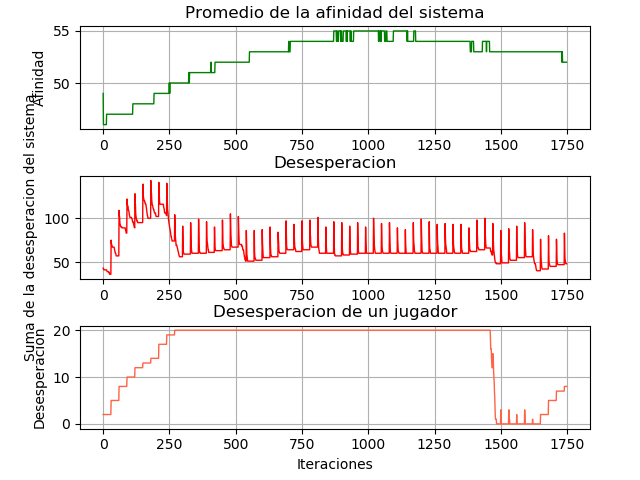
\includegraphics[width=0.7\linewidth]{Graficas_It_1_snMuertes}
	\caption{Comportamiento de una ejecución del sistema sin muertes.}
	\label{fig:graficasit1snmuertes}
\end{figure}

En la figura \ref{fig:graficasit2snmuertes} podemos ver otras gráficas de una ejecución distinta, esto porque ya que usamos números aleatorios es importante 
ver distintos comportamientos del sistema. 
Podemos notar en la grafica de la afinidad del sistema que la afinidad comienza a 
subir al final de la ejecución, más que en la ejecución anteriormente explicada. 
Se puede notar que también hay un valle marcado, esto se puede dar porque como se 
explicó, si agentes que se llevan mal interactúan, la afinidad decrece para ambos. 
La desesperación del sistema comienza my alta y sin embargo, conforme transcurren 
las iteraciones va descendiendo hasta que se queda casi en ceros para todos los 
jugadores. Una cosa a notar es que se pueden ver picos muy pronunciados en la 
gráfica, esto es porque como cada cierto número de iteraciones hay incentivos para
todos los jugadores, entonces aumenta drásticamente la suma. Una cosa interesante a 
notar es que cuando decrementa la afinidad la desesperación aumenta alrededor del 
mismo lapso de tiempo, esto se puede dar porque los promedios de afinidad de los
jugadores decrecio al punto en el que no era suficiente para decrementar la 
desesperación.
Por último en la gráfica de la desesperación de un jugador, podemos ver como de nuevo se mantiene en valores de 20 durante mucho tiempo, lo cual coincie con los valores de alrededor de 50 en la desesperación del sistema, y sin embargo alrededor
de la iteración 1500 el valor disminuye hasta que comienza a estancarse en casi cero.

\begin{figure}[h!]
	\centering
	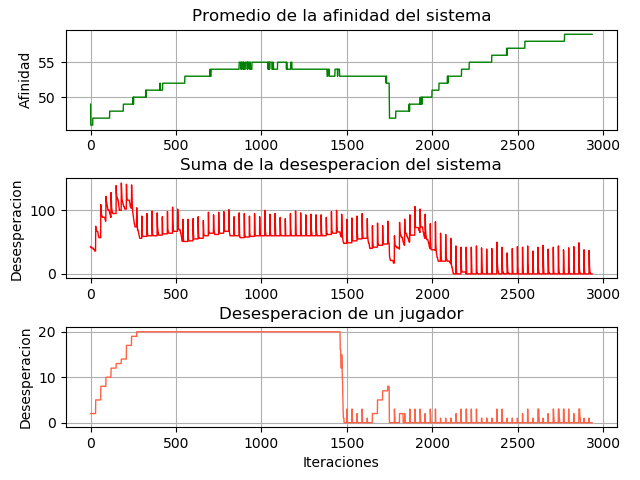
\includegraphics[width=0.7\linewidth]{Graficas_It_2_snMuertes}
	\caption{Comportamiento de otra ejecución del sistema sin muertes aún.}
	\label{fig:graficasit2snmuertes}
\end{figure}

Se ejecutó varias veces esta modalidad de sistema y siempre terminaba convergiendo
a una afinidad positiva y una desesperación de casi cero (valores entre 0 y 3 por 
los incentivos), esto nos puede dar una visión de que después de mucho convivir el entorno puede ser positivo a pesar de que se intente influir de manera negativa.

Después de esta experimentación se procedió a experimentar con el sistema completo, 
es decir, el modelo con todas las fases implementadas y también se obtuvieron 
resultados interesantes. En la figura \ref{fig:graficait7cnmuertes} podemos ver 4 
gráficas de una ejecución sobre una retícula de 20*20 y 20 agentes, cada línea azul 
representa un cambio de fase, es decir, una transición entre la fase 0 a 1, fase 1 
a 2 o fase 2 a 0. Se puede observar que el promedio de la afinidad en general 
desciende a diferencia de las gráficas anteriores, esto es poque con cada muerte
los jugadores que eran afines a los fallecidos son afectados en sus niveles de 
afinidad ya que esos valores se pierden, esto también contribuye a una gran 
perturbación en la desesperación ya que al descender el promedio un jugador puede
que ya no pueda bajar su nivel de desesperación. Esto se puede notar alrededor de 
las iteraciones 200 a 800 donde hay muchas muertes y muchos cambios de fase, 
se puede notar como el número de jugadores decrementa rápidamente junto con el 
promedio de afinidad. Los niveles de desesperación del sistema si bien no aumentan,
estos no descienden tan rápidamente. En la tercera gráfica podemos ver cómo se 
comporta el nivel de desesperación de un jugador, podemos ver que su nivel de 
desesperación decrementaba hasta que comenzaron algunas muertes y entonces el nivel
del jugador llego a 20 y se mantuvo varias iteraciones así, al final podemos ver que
el nivel desciende bruscamente, esto se debe a que el jugador falleció durante la 
ejecución. 

\begin{figure}[h!]
	\centering
	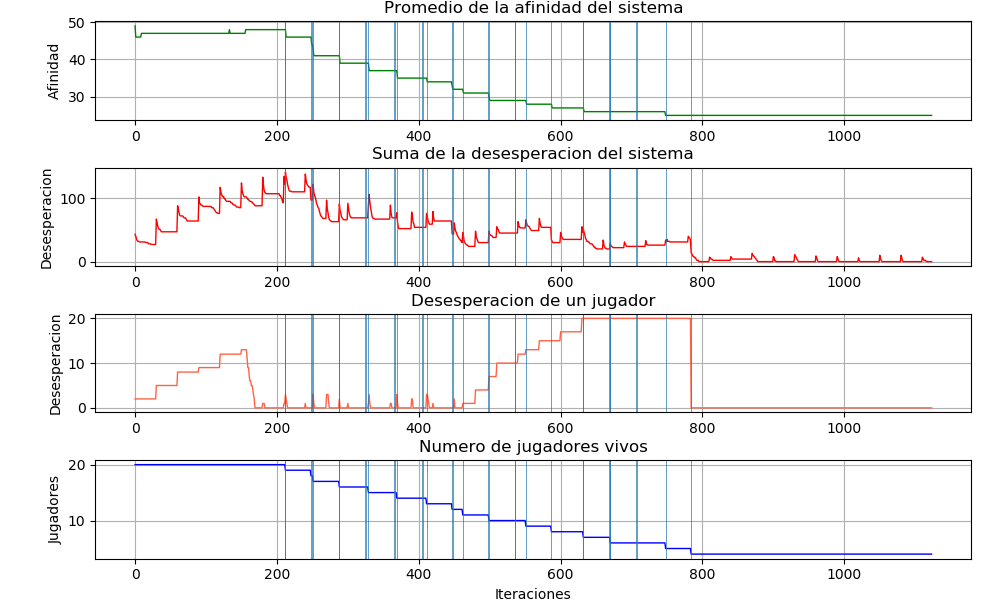
\includegraphics[width=0.7\linewidth]{Grafica_It_7cnMuertes}
	\caption{Grafica de una ejecución del sistema.}
	\label{fig:graficait7cnmuertes}
\end{figure}

Si observamos atentamente las gráficas podemos notar que al final de la ejecución tenemos un nivel de afinidad bajo a comparación a las ejecuciones anteriores, un 
nivel de desesperación en el sistema bajo también pero nos quedaron 2 jugadores 
vivos únicamente. Una cosa que se notó desde la primera iteración es que por
los criterios a la hora de pasar de fase y en el juicio al no dar opción
a disminuir la desesperación durante la fase 1 y 2 si hay varios jugadores
con nivel de 20 estos jugadores comienzan a asesinar de uno en uno, es decir, en 
cuando se vuelve a la fase 0 un nuevo jugador asesina inmediatamente y si por otro 
lado en el juicio no se encuentra al culpable, al regresar a la fase 0 el asesino 
con una alta probabilidad vuelve a asesinar.

En otra ejecución con los mismos parámetros que en la anterior obtenemos la figura 
\ref{fig:graficasit5cnmuertes} podemos notar de nuevo como la afinidad del sistema 
desciende mucho y se mantiene en valores de 40 en promedio aproximadamente, se puede
notar que de nuevo este valor comienza a decrementar cuando comienzan a ocurrir
las muertes entre jugadores. La suma de la desesperación si bien no aumenta, se 
mantiene alrededor de ciertos valores. La gráfica del valor para un jugador seleccionado se mantiene alrededor de valores bajos y no se ve muy afectado por las muertes. 

\begin{figure}[h!]
	\centering
	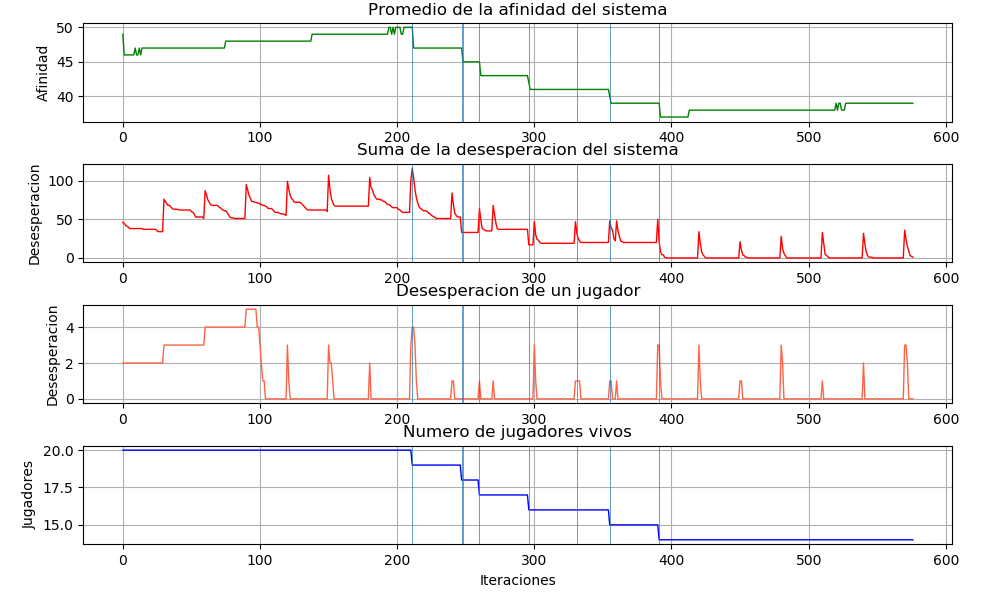
\includegraphics[width=0.7\linewidth]{Graficas_It_5cnMuertes}
	\caption{Segunda ejecución del sistema.}
	\label{fig:graficasit5cnmuertes}
\end{figure}

Se puede notar que en esta ejecución hay más sobrevivientes y que la etapa 
de caos dura mucho menos que en la ejecución anterior en la cual casi todos 
fallecieron. Una cosa a notar es que al final de la ejecución el sistema llegó
a un equilibrio en el que la afinidad se mantuvo en un valor y la desesperación se mantuvo en valores bajos también, haciendo que los jugadores ya no se asesinaran a
pesar de los incentivos que se manifestaban.


 
Un tercer comportamiento interesante que se observó fue uno en el que los jugadores 
casi desde el inicio tienen una afinidad alta y los incentivos no los afectan en 
gran medida. Esto se puede observar en la figura \ref{fig:graficasit6cnmuertes} 
donde desde un inicio se puede ver que hay una afinidad muy alta y esta comienza a 
incrementar rápidamente, esto se debe a la buena afinidad que había entre los 
jugadores. La desesperación también decrementa desde un inicio rápidamente hasta 
llegar a valores muy cercanos al cero en menos de 300 iteraciones. Al observar la tercera gráfica podemos corroborar como el jugador decrementa su desesperación 
velozmente hasta llegar a valores de casi cero y lograr contrarestar los incentivos
en unas cuantas iteraciones. 

\begin{figure}[h!]
	\centering
	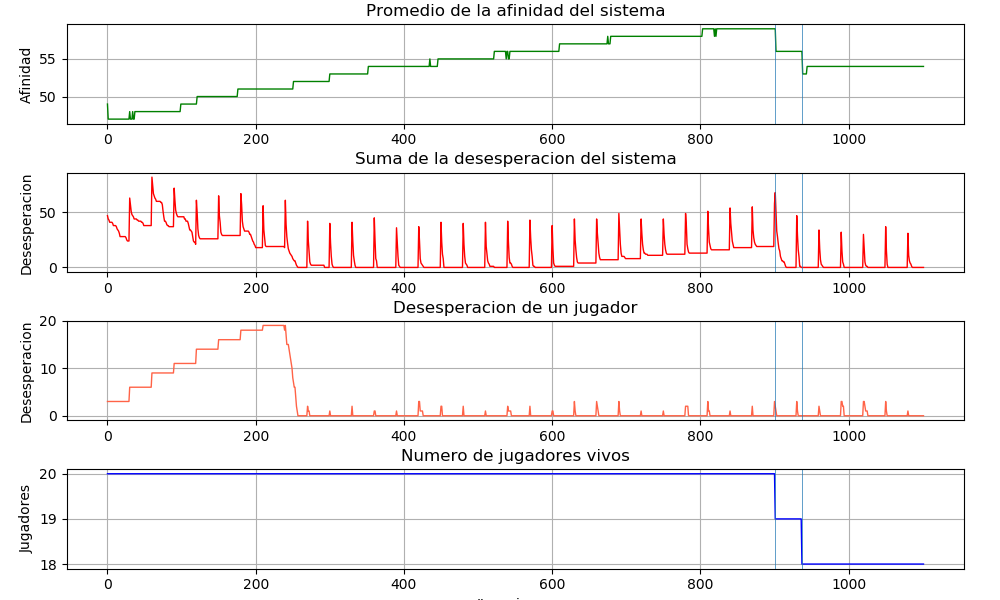
\includegraphics[width=0.7\linewidth]{Graficas_It_6cnMuertes}
	\caption{Ejecución del sistema con 20 jugadores sobre una retícula de 20*20.}
	\label{fig:graficasit6cnmuertes}
\end{figure}

Se puede observar también que solo ocurre un solo asesinato en la cuarta gráfica y 
después de esto no ocurren más, la afinidad converge a un valor así como la 
desesperación del sistema y aunque se nota que las muertes del asesino y la víctima
afectaron en la afinidad, el sistema fue capaz de equilibrarse.
 
\section{Conclusiones}

Después de haber ejecutado el sistema completo varias veces se puede concluir que en
general los jugadores convergen a un valor de paz a pesar de que ocurran algunos 
asesinatos (alrededor de 4). De hecho es muy rara una iteración en la que los 
jugadores se maten demasiado como en \ref{fig:graficait7cnmuertes}, de 
aproximadamente de 15 iteraciones en una ocurre un fenónmeno similar. Por lo 
anterior se podría concluir que el sistema llega a una cooperación entre todos y 
por más que los intenten orillar a matar, dada la cooperación grupal, esto es casi
imposible.


\begin{thebibliography}{7}
	
	\bibitem{WDil}
	Dilema del prisionero, en \emph{Wikipedia} consultado en junio 6,2019 desde \url{https://es.wikipedia.org/wiki/Dilema_del_prisionero}. 
\end{thebibliography} 

\end{document}
